\section{Illustrative Examples}

\begin{figure*}
    \centering
    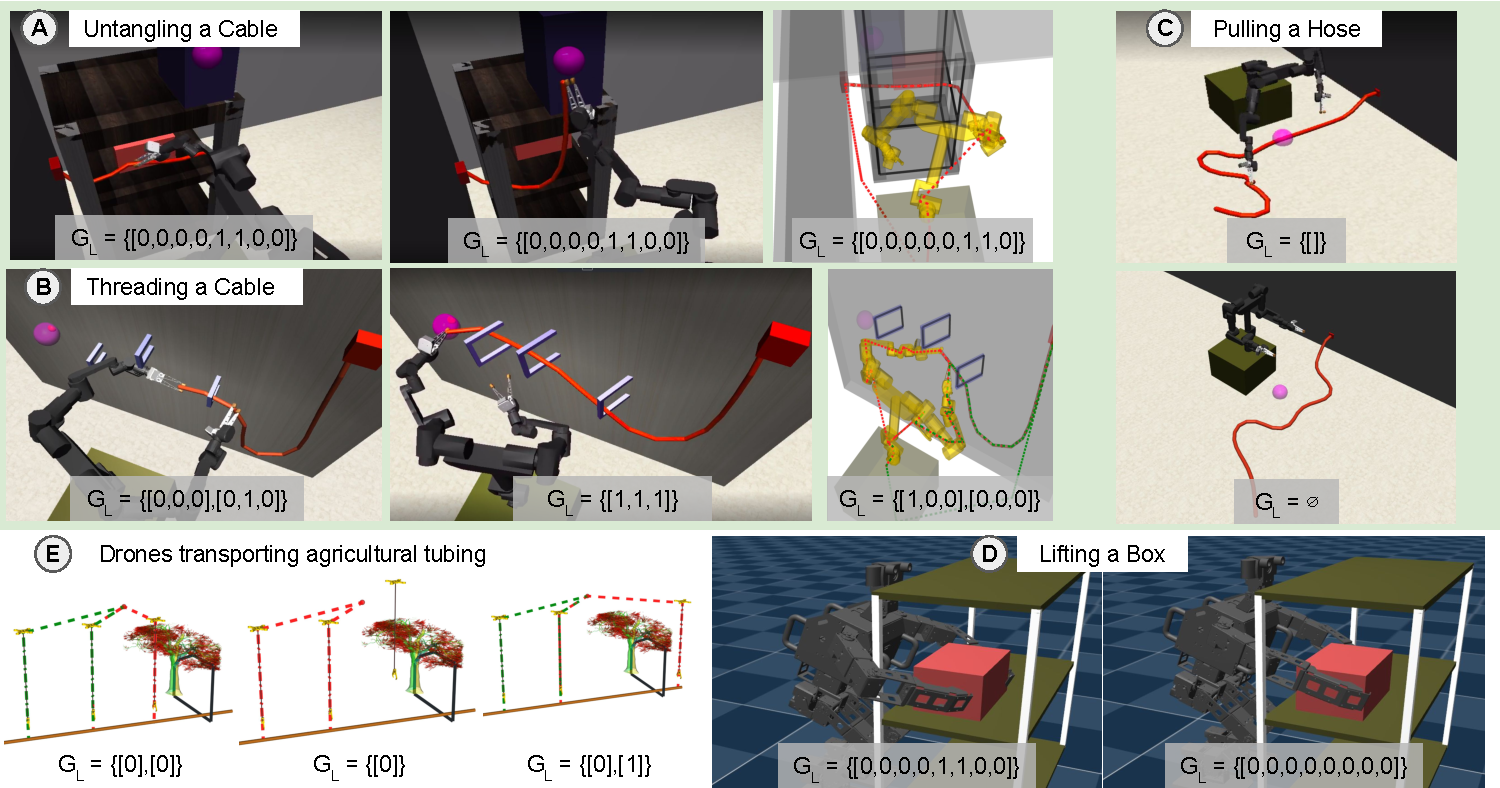
\includegraphics[width=\linewidth]{Chap5/images/examples.pdf}
    \caption{Example scenes and their $\sig$ values. The Panel in green shows environments where we use the \signature{} in planning. Panels D and E are additional examples where the \signature{} may be useful.}
    \label{fig:examples}
\end{figure*}

Figure \ref{fig:examples} shows a variety of robotic systems for which we can compute the \signature{}. The upper group show environments where we apply our planning methods. The lower group are examples where we believe the \signature{} would be useful, but do not conduct evaluations. In panel A, the second and third images show how the signature is invariant to smooth deformations, such as a change in object shape or sliding the arm along the DOO. The drones example in section C shows how we can create virtual connections between objects which are not physically connected. This allows the planner to distinguish between E1 and E3, in which the third drone is lifting the hose from different sides of the tree branch.